%%%%%%%%%%%%%%%%%%%%%%%%%%%%%%%%% LAB-5 %%%%%%%%%%%%%%%%%%%%%%%%%%%%%%%%%%
%>>>>>>>>>>>>>>>>>>>>>>>>>> ПЕРЕМЕННЫЕ >>>>>>>>>>>>>>>>>>>>>>>>>>>>>>>>>>>
%>>>>> Информация о кафедре
%\newcommand{\year}{2021 г.}  % Год устанавливается автоматически
\newcommand{\city}{Санкт-Петербург}  %  Футер, нижний колонтитул на титульном листе
\newcommand{\university}{Национальный исследовательский университет ИТМО}  % первая строка
\newcommand{\department}{Факультет программной инженерии и компьютерной техники}  % Вторая строка
\newcommand{\major}{Направление системного и прикладного программного обеспечения}  % Треьтя строка
%<<<<< Информация о кафедре

%>>>>> Назание работы
\newcommand{\reporttype}{ОТЧЕТ ПО ЛАБОРАТОРНОЙ РАБОТЕ} % тип работы, (главный заголовок титульного листа)
\newcommand{\lab}{Лабораторная работа}          % вид работы
\newcommand{\labnumber}{№ 3}                    % порядковый номер работы
\newcommand{\subject}{Программирование}         % учебный предмет
\newcommand{\labtheme}{Принципы ООП}            % Тема лабораторной работы
\newcommand{\variant}{№ 1234510}                % номер варианта работы

\newcommand{\student}{Тюрин Иван Николаевич}    % определение ФИО студента
\newcommand{\studygroup}{P3110}                 % определение учебной группы 
\newcommand{\teacher}{% принимающий
    Письмак А. Е.,\\[1mm]% ФИО лектора
    Сорокин Р. Б.% ФИО практика
}
%<<<<<<<<<<<<<<<<<<<<<<<<<< ПЕРЕМЕННЫЕ <<<<<<<<<<<<<<<<<<<<<<<<<<<<<<<<<<<


%>>>>>>>>>>>>>>>>>>>>>> ПРЕАМБУЛА >>>>>>>>>>>>>>>>>>>>>>>>>

%>>>>>>>>>>>>>>>>>> ПРЕАМБУЛА >>>>>>>>>>>>>>>>>>>>
\documentclass[14pt,final,oneside]{extreport}
%>>>>> Разметка документа
\usepackage[a4paper, mag=1000, left=3cm, right=1.5cm, top=2cm, bottom=2cm, headsep=0.7cm, footskip=1cm]{geometry} % По ГОСТу: left>=3cm, right=1cm, top=2cm, bottom=2cm,
\linespread{1} % межстройчный интервал по ГОСТу := 1.5
%<<<<< Разметка документа

%>>>>> babel c языковым пакетом НЕ должны быть первым импортируемым пакетом
\usepackage[utf8]{inputenc}
\usepackage[T1,T2A]{fontenc}
\usepackage[russian]{babel}
%<<<<<

%\usepackage{cmap} %поиск в pdf

%>>>...>> прочие полезные пакеты
\usepackage{amsmath,amsthm,amssymb}
\usepackage{mathtext}
\usepackage{indentfirst}
\usepackage{graphicx}
\graphicspath{{/home/ivan/itmo/informatics/latex}}
\DeclareGraphicsExtensions{.pdf,.png,.jpg}
%\usepackage{bookmark}

\usepackage[dvipsnames]{xcolor}
\usepackage{hyperref}  % Использование ссылок
\hypersetup{%  % Настройка разметки ссылок
    colorlinks=true,
    linkcolor=blue,
    filecolor=magenta,      
    urlcolor=magenta,
    %pdftitle={Overleaf Example},
    %pdfpagemode=FullScreen,
}

%>>>>> Использование листингов
\usepackage{listings} 
\usepackage{caption}
\DeclareCaptionFont{white}{\color{white}} 
\DeclareCaptionFormat{listing}{\colorbox{gray}{\parbox{\textwidth}{#1#2#3}}}

\captionsetup[lstlisting]{format=listing,labelfont=white,textfont=white} % Настройка вида описаний
\lstset{  % Настройки вида листинга
inputencoding=utf8, extendedchars=\true, keepspaces = true, % поддержка кириллицы и пробелов в комментариях
language=Pascal,            % выбор языка для подсветки (здесь это Pascal)
basicstyle=\small\sffamily, % размер и начертание шрифта для подсветки кода
numbers=left,               % где поставить нумерацию строк (слева\справа)
numberstyle=\tiny,          % размер шрифта для номеров строк
stepnumber=1,               % размер шага между двумя номерами строк
numbersep=5pt,              % как далеко отстоят номера строк от подсвечиваемого кода
backgroundcolor=\color{white}, % цвет фона подсветки - используем \usepackage{color}
showspaces=false,           % показывать или нет пробелы специальными отступами
showstringspaces=false,     % показывать илигнет пробелы в строках
showtabs=false,             % показывать или нет табуляцию в строках
frame=single,               % рисовать рамку вокруг кода
tabsize=2,                  % размер табуляции по умолчанию равен 2 пробелам
captionpos=t,               % позиция заголовка вверху [t] или внизу [b] 
breaklines=true,            % автоматически переносить строки (да\нет)
breakatwhitespace=false,    % переносить строки только если есть пробел
escapeinside={\%*}{*)}      % если нужно добавить комментарии в коде
}
%<<<<< Использование листингов

\sloppy % Решение проблем с переносами (с. 119 книга Львовского)
\emergencystretch=25pt


%>>>>>>>>>>>>>>>> КОМАНДЫ {Для соответствия ГОСТ} >>>>>>>>>>>>>>

\newcommand\Chapter[2]{
    % Принимает 2 аргумента - название главы и дополнительный заголовок 
    \refstepcounter{chapter}
    \chapter*{
        \begin{huge}
        % Отключена нумерация глав в тексте:
        %:=% \textbf{\chaptername\ \arabic{chapter}\\}
        \textbf{#1}
        \end{huge}
        \raggedright
        \bigskip \bigskip
        #2
    }
    % Отключена нумерация для chapter в toc (table of contents), т.е. Оглавлении (Содержании):
    %:=% \addcontentsline{toc}{chapter}{\arabic{chapter}. #1}
    % Представление главы в содержании:
    \addcontentsline{toc}{chapter}{#1 #2} 
}


\newcommand\Section[1]{
    % Принимает 1 аргумент - название секции
    \refstepcounter{section}
    \section*{%
        \raggedright
        % Отключена дополнительная нумерация chapter в section в тексте документа:
        %:=% \arabic{chapter}.\arabic{section}. #1}
        % Отключена любая нумарация section в тексте документа: (убрать \arabic{section}, оставить название секции)
        \arabic{section}. #1
    }
    
    % Отключена дополнительная нумерация chapter в section в toc (table of contents) Оглавлении (Содержании):
    %:=% \addcontentsline{toc}{section}{\arabic{chapter}.\arabic{section}. #1}
    \addcontentsline{toc}{section}{\arabic{section}. #1} 
}


\newcommand\Subsection[1]{
    % Принимает 1 аргумент - название подсекции
    \refstepcounter{subsection}
    \subsection*{%
        \raggedright%
        % Отключена дополнительная нумерация chapter в section в тексте документа (можно добавить отступ с помощью \hspace*{12pt}):
        %:=% \arabic{chapter}.\arabic{section}.\arabic{subsection}. #1}
        \arabic{section}. \arabic{subsection}. #1
    }
    % Отключена дополнительная нумерация chapter в section в Оглавлении (Содержании):
    %\addcontentsline{toc}{subsection}{\arabic{chapter}.\arabic{section}.\arabic{subsection}. #1}
    \addcontentsline{toc}{subsection}{\arabic{subsection}. #1}
}


\newcommand\Figure[4]{
    % Принимает 4 аргумента - название файла изображения, ее размер в тексте, описание, лэйбл (псевдоним) 
        \refstepcounter{figure}
        \begin{figure}[h]
            \center{\includegraphics[width=#2]{#1}}
        \caption{#3}
        \label{fig:#4}
    \end{figure}
}

%<<<<<<<<<<<<<<<<<<<<<<<<<<<< КОМАНДЫ <<<<<<<<<<<<<<<<<<<<<<<<<<

%<<<<<<<<<<<<<<<<<<<<<< ПРЕАМБУЛА <<<<<<<<<<<<<<<<<<<<<<<<<



%%%%%%%%%%%%%%%%%%% СОДЕРЖИМОЕ ОТЧЕТА %%%%%%%%%%%%%%%%%%%%%
%>>>>>>>>>>>>>>> ''''''''''''''''''''''' >>>>>>>>>>>>>>>>>>
\begin{document}


%>>>>>>>>>>>>>>>> ОПРЕДЕЛЕНИЕ НАЗВАНИЙ >>>>>>>>>>>>>>>>>>>>
% Переоформление некоторых стандартных названий
%\renewcommand{\chaptername}{Лабораторная работа}
\renewcommand{\chaptername}{\lab\ \labnumber} % переименование глав
\def\contentsname{Содержание} % переименование оглавления
%<<<<<<<<<<<<<<<< ОПРЕДЕЛЕНИЕ НАЗВАНИЙ <<<<<<<<<<<<<<<<<<<<
% \setlength{\itemsep}{0pt} % установка расстояния между строчками в списках можно использовать локально внутри списка списке
% \setlength{\parskip}{0pt} % 
% \setlength{\parsep}{0pt}  % 

%>>>>>>>>>>>>>>>>> ТИТУЛЬНАЯ СТРАНИЦА >>>>>>>>>>>>>>>>>>>>>
%>>>>>>>>>>>>>>>>>>> ТИТУЛЬНЫЙ ЛИСТ >>>>>>>>>>>>>>>>>>>>>>>
\begin{titlepage}

    % Название университета
    \begin{center}
    \textsc{%
        \university\\[5mm]
        \department\\[2mm]
        \major\\
    }

    \vfill
    \vfill
    % Название работы
    \textbf{\reporttype\ \labnumber\\[3mm]
    курса <<\subject>> \\[6mm]
    по теме: <<\labtheme>>\\[3mm]
    Вариант \variant\\[20mm]
    }
    \end{center}


\hfill
% Информация об авторе работы и проверяющем
\begin{minipage}{.5\textwidth}
    \begin{flushright}
        
            
        Выполнил студент:\\[2mm] 
        \student\\[2mm]
        группа: \studygroup\\[5mm]

        Преподаватель:\\[2mm] 
        \teacher

    \end{flushright}
\end{minipage}

\vfill

    % Нижний колонтитул первой страницы
    \begin{center}
        \city, \the\year\,г.
    \end{center}

\end{titlepage}
%<<<<<<<<<<<<<<<<<<< ТИТУЛЬНЫЙ ЛИСТ <<<<<<<<<<<<<<<<<<<<<<<


%<<<<<<<<<<<<<<<<< ТИТУЛЬНАЯ СТРАНИЦА <<<<<<<<<<<<<<<<<<<<<


%>>>>>>>>>>>>>>>>>>>>> СОДЕРЖАНИЕ >>>>>>>>>>>>>>>>>>>>>>>>>
% Содержание
\tableofcontents
%<<<<<<<<<<<<<<<<<<<<< СОДЕРЖАНИЕ <<<<<<<<<<<<<<<<<<<<<<<<<


%%%%%%%%%%%%%%%%%%%%%%% КОД РАБОТЫ %%%%%%%%%%%%%%%%%%%%%%%%
%>>>>>>>>>>>>>>>>>>>'''''''''''''''''>>>>>>>>>>>>>>>>>>>>>
\newpage
\Chapter{\lab\ \labnumber}{\labtheme}{}

\Section{Задание варианта \variant}

\begin{center} , , , \end{center}
\noindent
\textbf{
   % Заглавное описание....:
   Заголовок
}

\textit{
    % Описание задания...
    Описание
}

\begin{itemize}
    \setlength{\itemsep}{0pt} % Сокращение межстрочных расстояний
    \setlength{\parskip}{0pt}
    \setlength{\parsep}{0pt} 
    \item 1
    \item 2
\end{itemize}

\begin{center} ' ' ' \end{center}

\newpage
\Section{Выполнение задания}
Что-то про задание

\Subsection{Листинги кода}
Листинг из файла \ref{lst:biblist}
\lstinputlisting[caption={Список источников},label={lst:biblist}]{./biblist.tex}

Листинг прямо в тексте \ref{lst:sql}
\begin{lstlisting}[caption={SQL},label={lst:sql}]
declare @t table(
  id int
)
\end{lstlisting}

Вставленное изображение с описанием и шириной по тексту.
\begin{figure}[H] % 'H' -- вставить тут же (подключен модуль), обычный вариант: 'htpb'
    \centering
    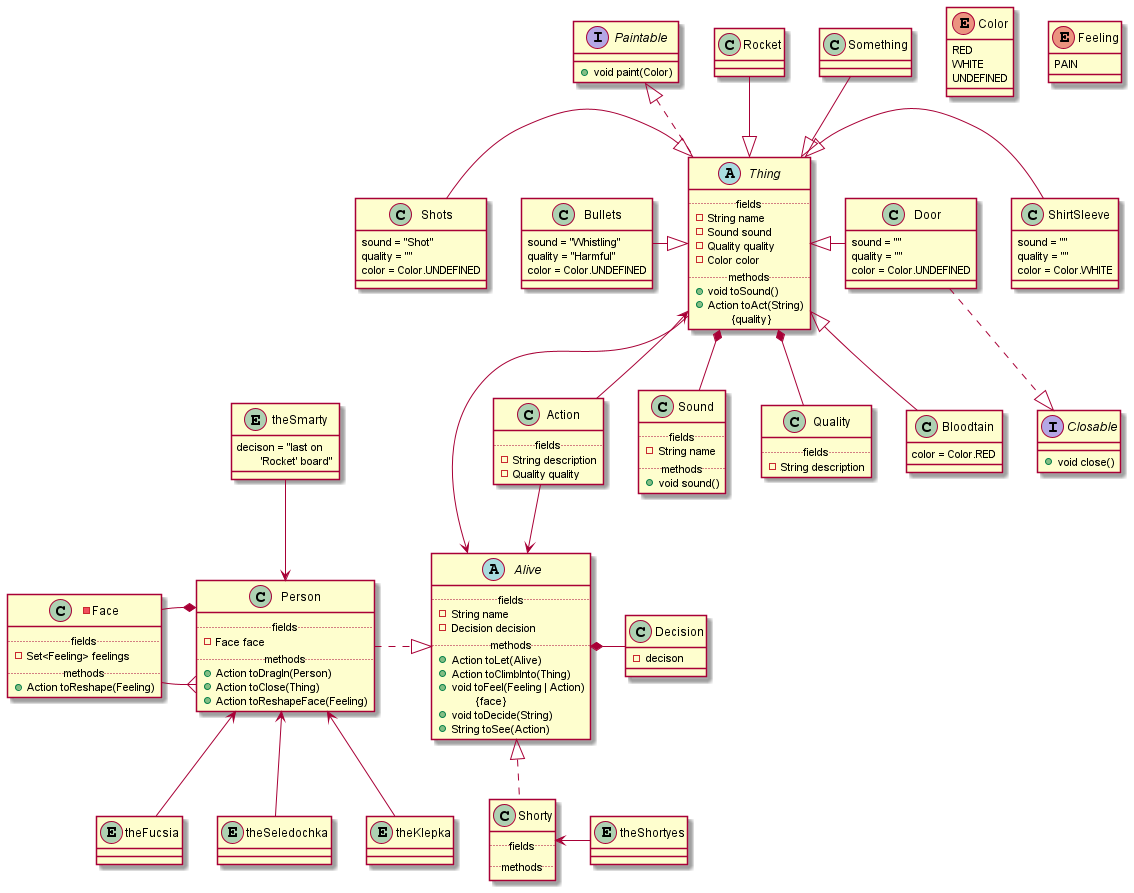
\includegraphics[width=\textwidth]{res/UML-class-diagram.png}
    \caption{Caption}
    \label{fig:enter-label}
\end{figure}


% Выполнение задания...

\Section{Вывод}
% Вывод... 
Ссылка \cite{itmocompmath} % -- из biblist
\newpage
%<<<<<<<<<<<<<<<<<<<<<< КОД РАБОТЫ <<<<<<<<<<<<<<<<<<<<<<<<


%>>>>>>>>>>>>>>>> СПИСОК ЛИТЕРАТУРЫ >>>>>>>>>>>>>>>>>>>>>>>
\begin{thebibliography}{}
\bibitem{itmocompmath} Cсылка на личный репозиторий GitHub: \url{https://github.com/e1turin/itmo-comp-math/tree/dev-lab-1/lab-1}\\
\end{thebibliography}  % Для соответсвия гост, придется доработать. Нужен файл .bib
%<<<<<<<<<<<<<<<<<<<< СПИСОК ЛИТЕРАТУРЫ <<<<<<<<<<<<<<<<<<<


\end{document}
%<<<<<<<<<<<<<<<< ,,,,,,,,,,,,,,,,,,,,,,, <<<<<<<<<<<<<<<<<
%<<<<<<<<<<<<<<<<<<< СОДЕРЖИМОЕ ОТЧЕТА <<<<<<<<<<<<<<<<<<<<
